\documentclass{article}
\usepackage[utf8]{inputenc}
\usepackage{float}
\usepackage[spanish]{babel}
\usepackage{graphicx}
\usepackage{listings}
\usepackage{color}
\usepackage{datetime}
\usepackage{csquotes}
\usepackage[table,xcdraw]{xcolor}
\documentclass[xcolor=table]{beamer}
\newdate{date}{30}{04}{2019}

\title{Tarea 5}
\author{Jesus Angel Patlán Castillo (5261)}
\date{\displaydate{date}}



\begin{document}

\definecolor{codegreen}{rgb}{0,0.6,0}
\definecolor{codegray}{rgb}{0.5,0.5,0.5}
\definecolor{codepurple}{rgb}{0.58,0,0.82}
\definecolor{backcolour}{rgb}{0.95,0.95,0.92}
 
\lstdefinestyle{mystyle}{
    backgroundcolor=\color{backcolour},   
    commentstyle=\color{codegreen},
    keywordstyle=\color{magenta},
    numberstyle=\tiny\color{codegray},
    stringstyle=\color{codepurple},
    basicstyle=\footnotesize,
    breakatwhitespace=false,         
    breaklines=true,                 
    captionpos=b,                    
    keepspaces=true,                 
    numbers=left,                    
    numbersep=5pt,                  
    showspaces=false,                
    showstringspaces=false,
    showtabs=false,                  
    tabsize=2
}
 
\lstset{style=mystyle}


\maketitle
En esta tarea se analizan las características de grafos que son generados por un algoritmo de generación de grafos proporcionado por librerías de Python, además de estudiar como estas características afectan el tiempo de ejecución al momento de obtener el flujo máximo entre dos nodos dentro del grafo. Los algoritmos se obtuvieron por medio de la librería NetworkX \cite{NetworkX} de Python \cite{Python}, la librería Matplotlib \cite{Matplotlib} es utilizada para generar las gráfica de correlación entre los efectos estudiados. El código empleado se obtuvo consultando la documentación oficial de la librería NetworkX \cite{NetworkXD}. Las imágenes y el código se encuentran disponibles directamente en mi repositorio \cite{JAPC}.

\section{Metodología}
Basándonos en las tareas anteriores, se decide utilizar de algoritmo de generador de grafos de llamado grafo de cavernícola conexo, el cual tiene una mayor aplicación para el problema de flujo máximo dado que es posible representar cada cluster de nodos como una isla en la que se necesita transportar recursos a otro cluster. Además, tenemos que el algoritmo de flujo máximo que utilizaremos será el tradicional flujo máximo entre dos nodos, dado que fue el algoritmo que mostró un mejor desempeño en tiempo de ejecución. Para una mejor visualización se eligió el algoritmo de acomodo resorte, el cual da una mejor visualización de los nodos y las aristas del grafo.
Para las pruebas, se crearon 5 instancias distintas de grafo de cavernícola conexo, los cuales se muestran a continuación:
\begin{figure}[H]
    
\includegraphics[width=\textwidth]{grafo-1}
    \caption{Grafo 1}
    \label{fig:matriz}
\end{figure}
\begin{figure}[H]
    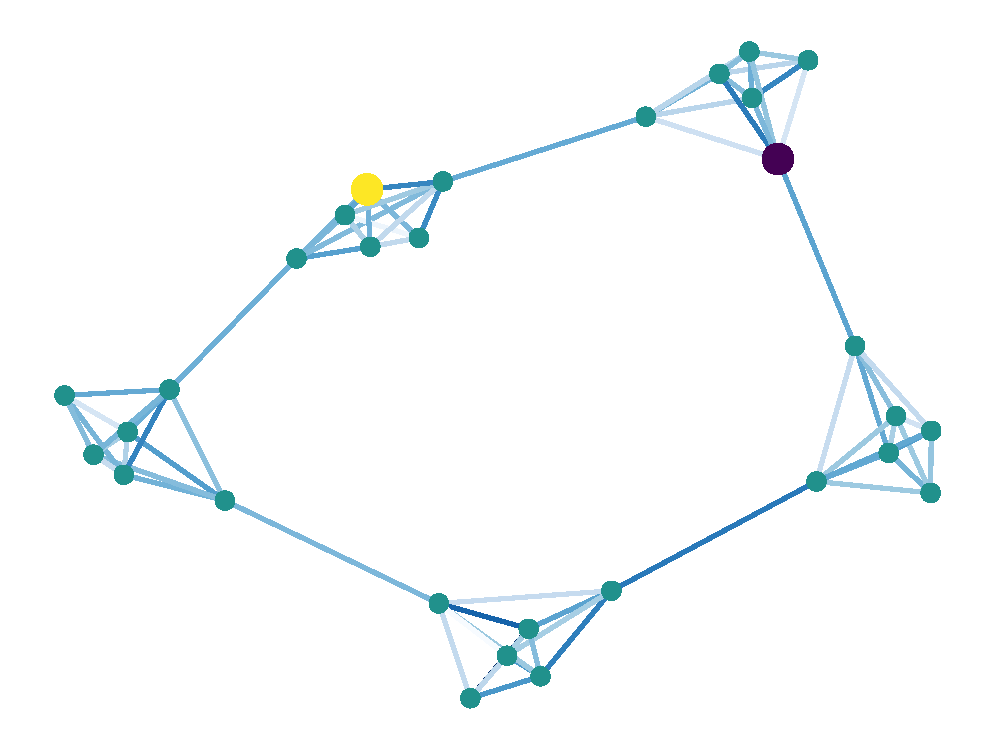
\includegraphics[width=\textwidth]{grafo-2}
    \caption{Grafo 2}
    \label{fig:matriz}
\end{figure}
\begin{figure}[H]
    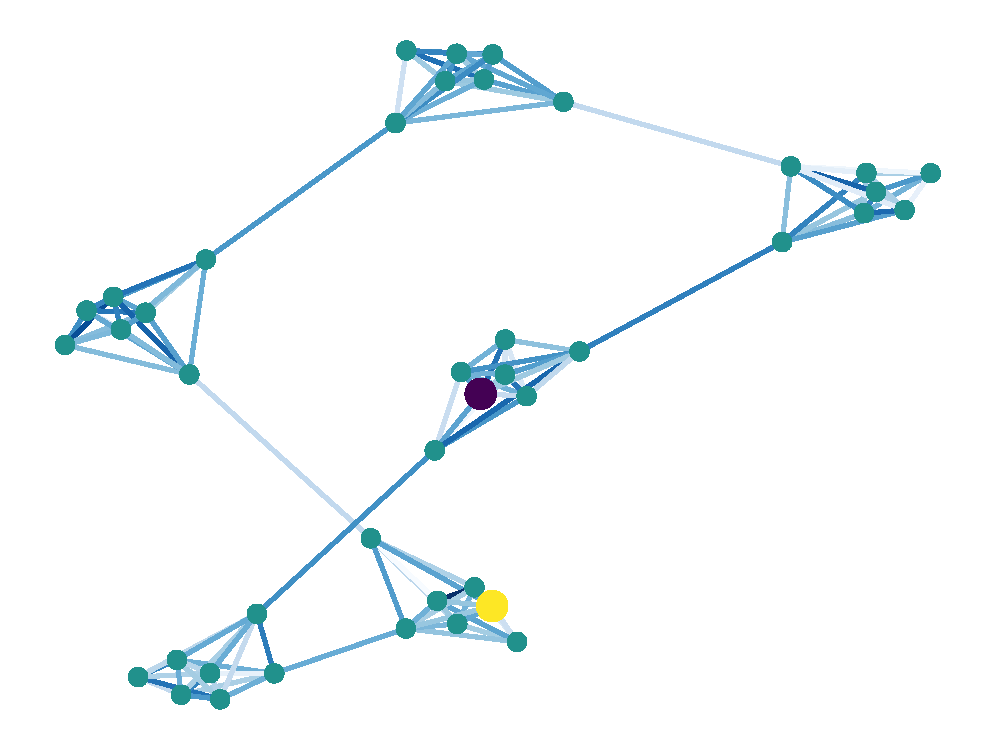
\includegraphics[width=\textwidth]{grafo-3}
    \caption{Grafo 3}
    \label{fig:matriz}
\end{figure}
\begin{figure}[H]
    
\includegraphics[width=\textwidth]{grafo-4}
    \caption{Grafo 4}
    \label{fig:matriz}
\end{figure}
\begin{figure}[H]
    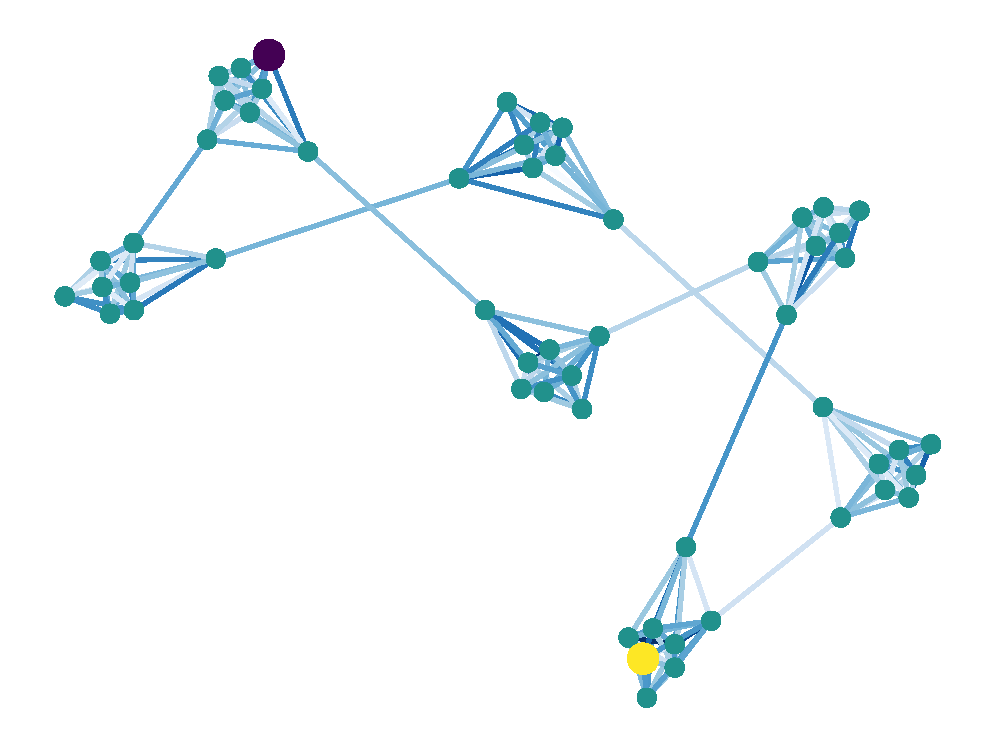
\includegraphics[width=\textwidth]{grafo-5}
    \caption{Grafo 5}
    \label{fig:matriz}
\end{figure}
Para cada grafo, señalamos un nodo fuente (en amarillo) y un nodo sumidero (en negro) de ejemplo para el problema de flujo máximo, además que resaltamos cada arista con un tono de azul más oscuro cuanto mayor sea el peso que tenga. Para cada uno de los grafos, se realizaron distintas pruebas intercambiando los nodos fuente-sumidero para determinar el rendimiento del algoritmo de flujo máximo. Además, a cada grafo se le determinan 5 características:
\begin{itemize}
\item Distribución de grado: Es el número de aristas asociadas a un nodo.
\item Coeficiente de agrupamiento: Determina que tanto un nodo esta asociado a sus nodos vecinos.
\item Centralidad de cercanía: Determina que tan cercano o alejado esta un nodo con respecto a los demás nodos vecinos.
\item Centralidad de carga: Determina el número de caminos más cortos que se pasan a través del nodo.
\item Excentricidad: Determina la longitud máxima que hay entre el nodo y otro nodo del grafo.
\item PageRank: Similar a la distribución de grado, pero da distinto pesos a las aristas de acuerdo al grado que tenga el nodo al que se conecta.
\end{itemize}
En base a estas 5 características, se realiza una prueba ANOVA para determinar como influyen estos en el tiempo de ejecución del algoritmo.
Un ejemplo aplicando el flujo máximo en cada grafo se muestra a continuación, donde se muestran solamente las aristas por donde el flujo se distribuye:
\begin{figure}[H]
    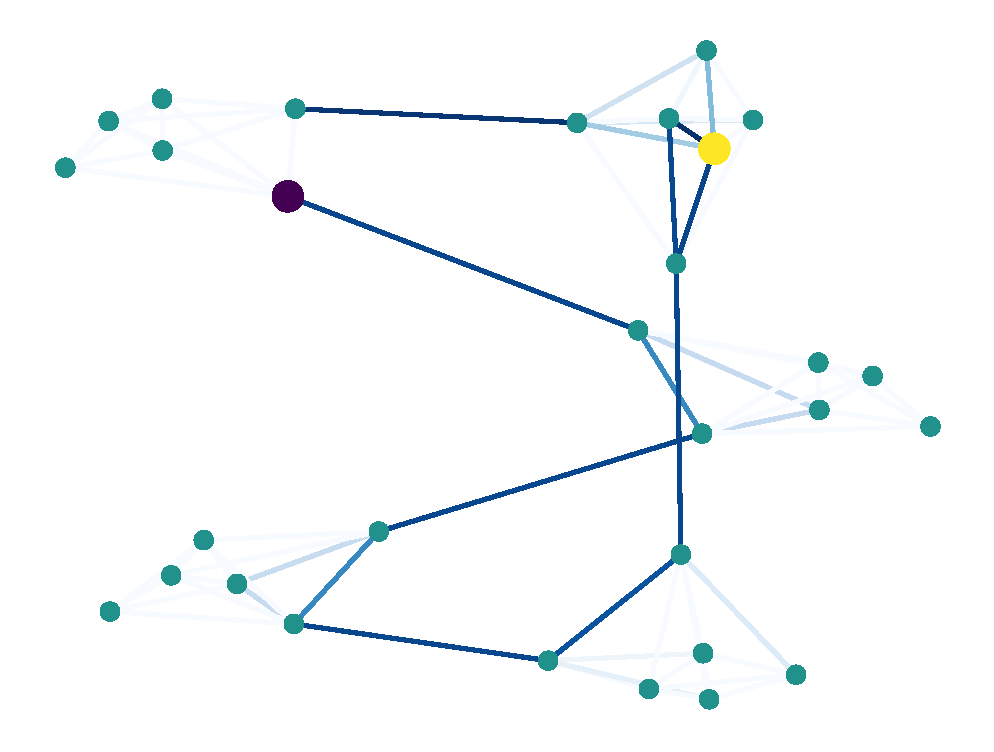
\includegraphics[width=\textwidth]{res-1}
    \caption{Grafo 1}
    \label{fig:matriz}
\end{figure}
\begin{figure}[H]
    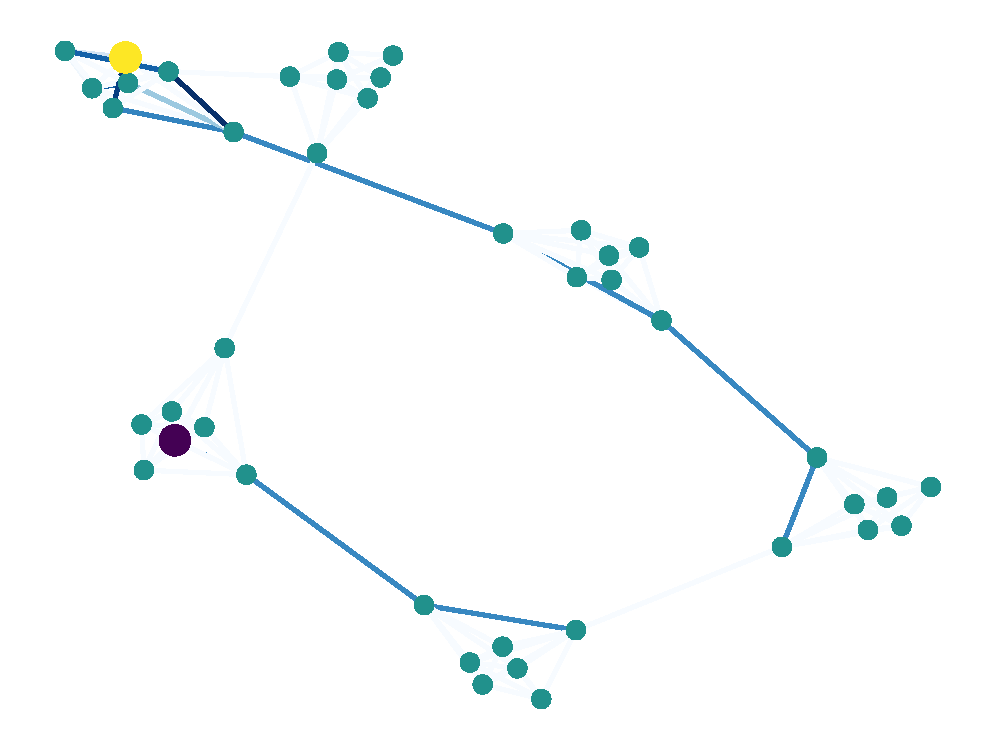
\includegraphics[width=\textwidth]{res-2}
    \caption{Grafo 2}
    \label{fig:matriz}
\end{figure}
\begin{figure}[H]
    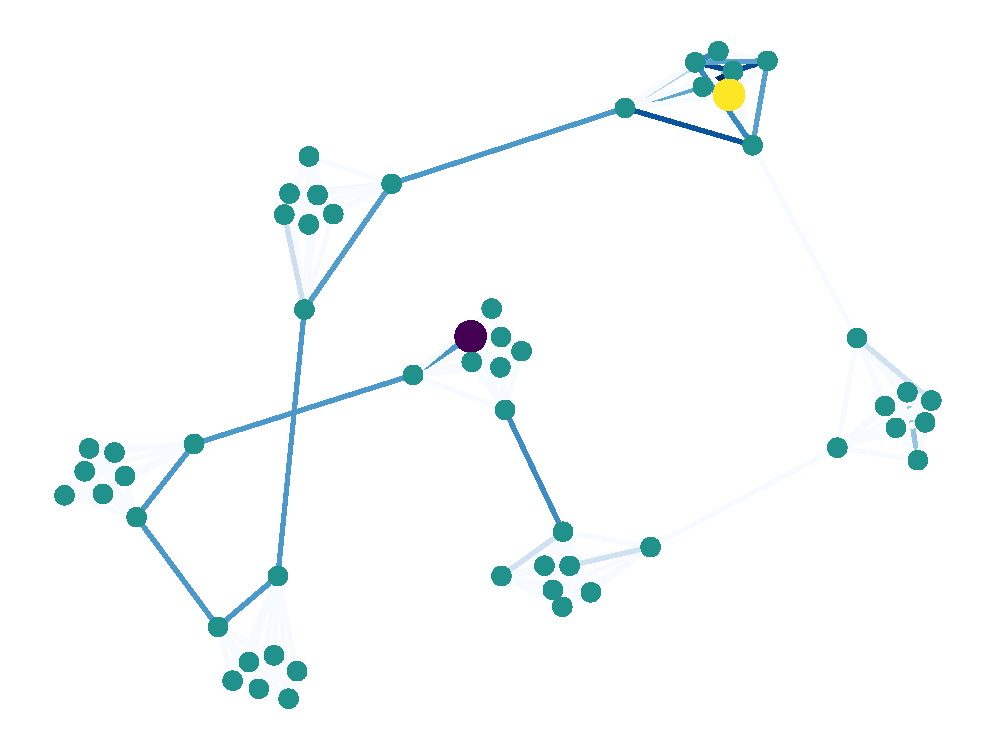
\includegraphics[width=\textwidth]{res-3}
    \caption{Grafo 3}
    \label{fig:matriz}
\end{figure}
\begin{figure}[H]
    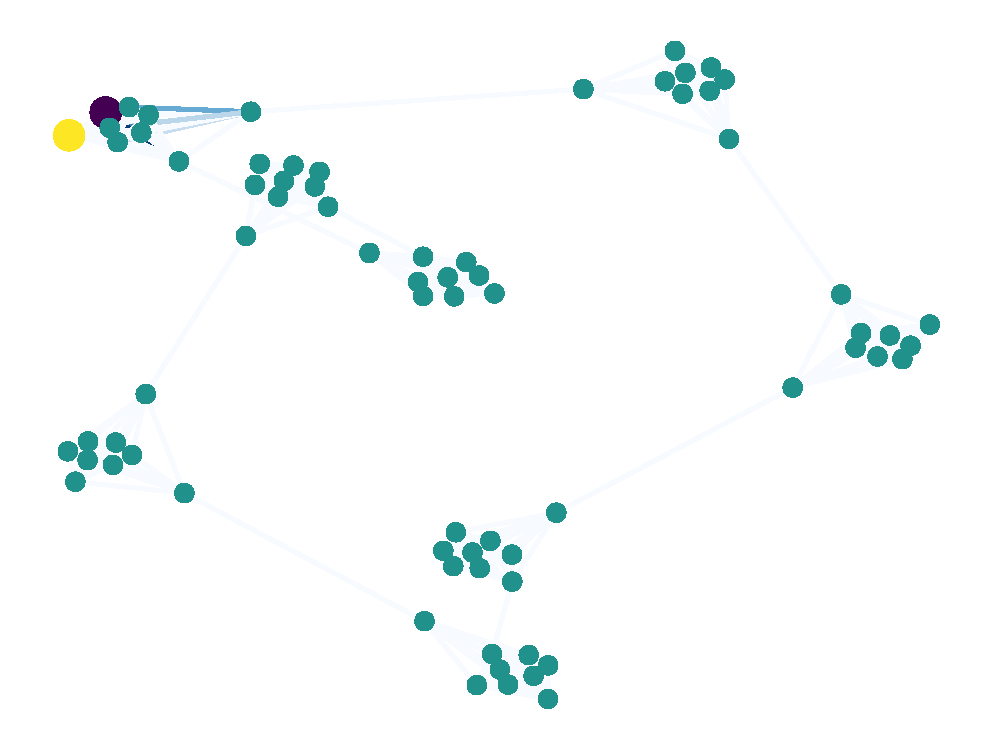
\includegraphics[width=\textwidth]{res-4}
    \caption{Grafo 4}
    \label{fig:matriz}
\end{figure}
\begin{figure}[H]
    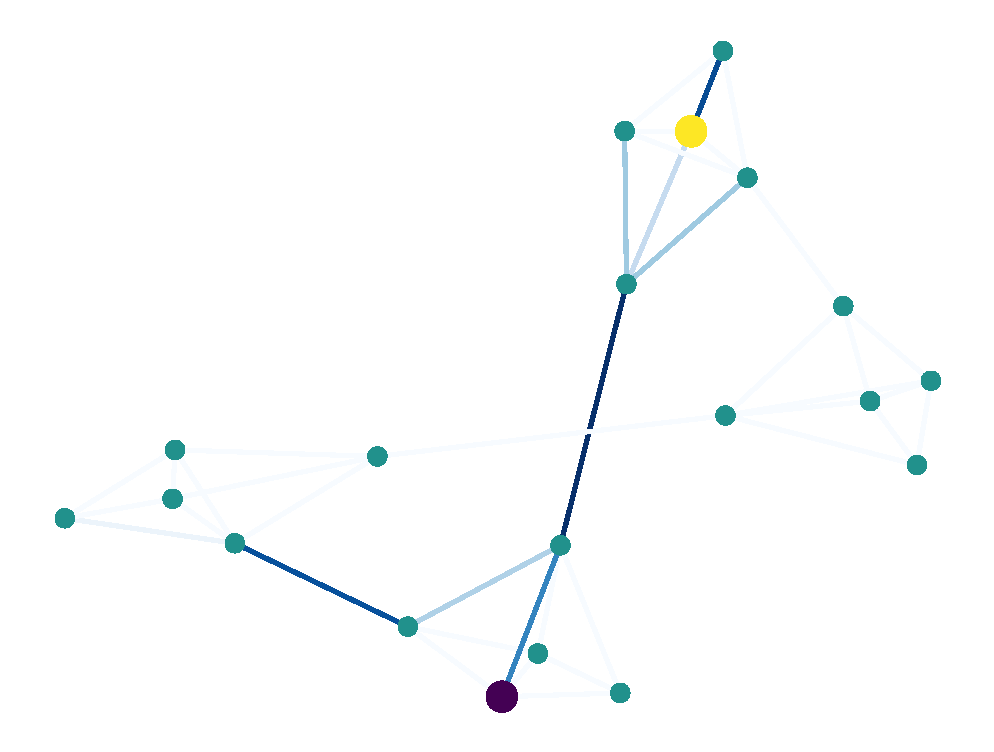
\includegraphics[width=\textwidth]{res-5}
    \caption{Grafo 5}
    \label{fig:matriz}
\end{figure}
Este proceso se realizó en una laptop con las siguientes características:
\begin{itemize}
\item{Procesador}: Intel Core i7-7500U 2.7GHz
\item{Memoria RAM}: 16GB 
\item{Sistema Operativo}: Windows 10 64 bits
\end{itemize}

\section{Resultados}
Estas son las características encontradas de las instancias de grafos:

\subsection{Grado de nodos}
\begin{figure}[H]
    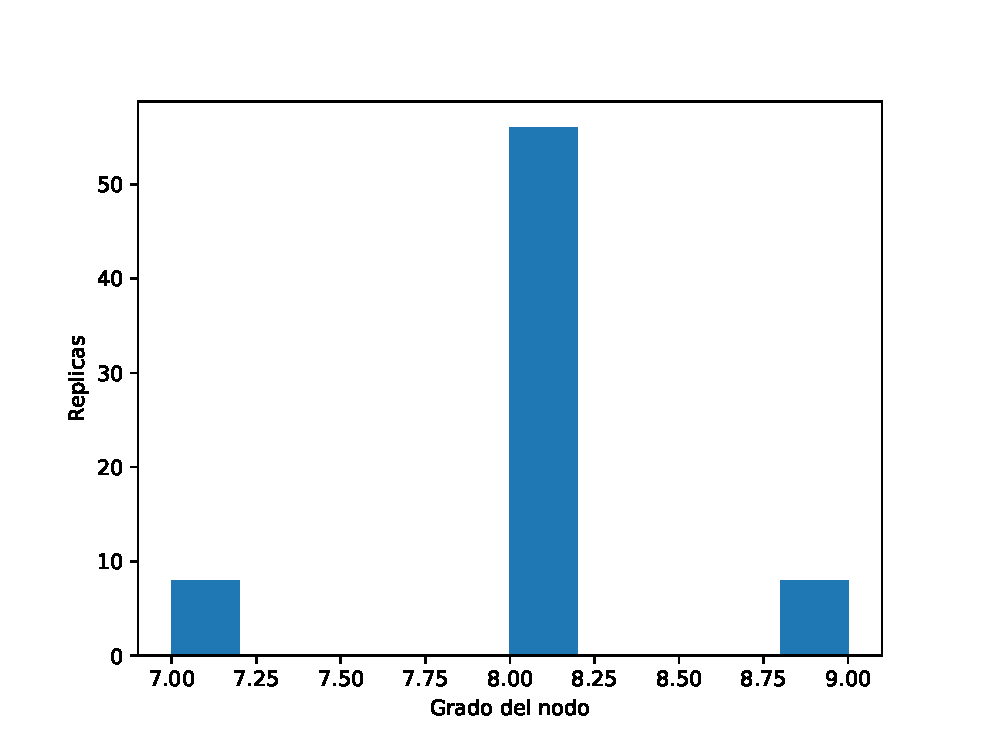
\includegraphics[scale=0.6]{hist-grados-1}
    \caption{Grafo 1}
    \label{fig:matriz}
\end{figure}
\begin{figure}[H]
    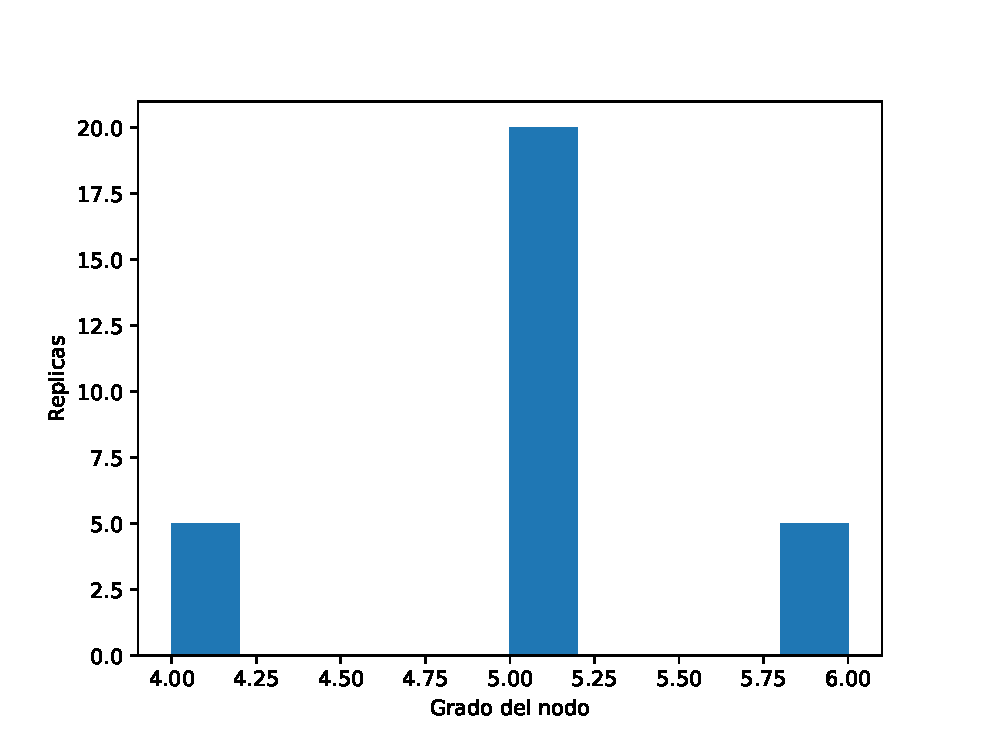
\includegraphics[scale=0.6]{hist-grados-2}
    \caption{Grafo 2}
    \label{fig:matriz}
\end{figure}
\begin{figure}[H]
    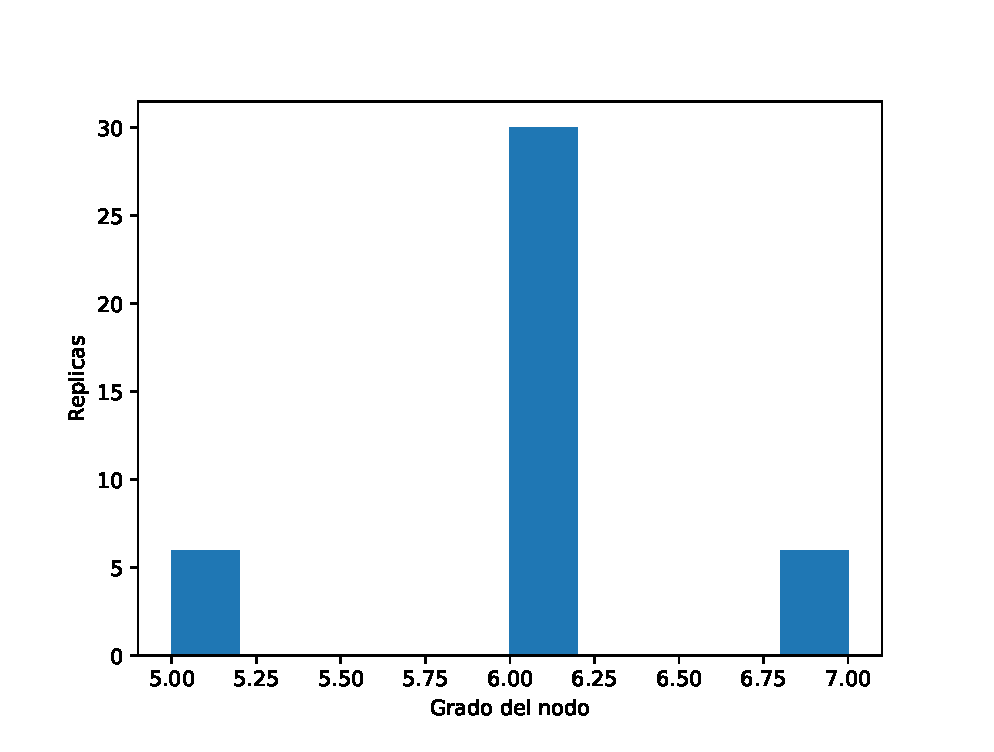
\includegraphics[scale=0.6]{hist-grados-3}
    \caption{Grafo 3}
    \label{fig:matriz}
\end{figure}
\begin{figure}[H]
    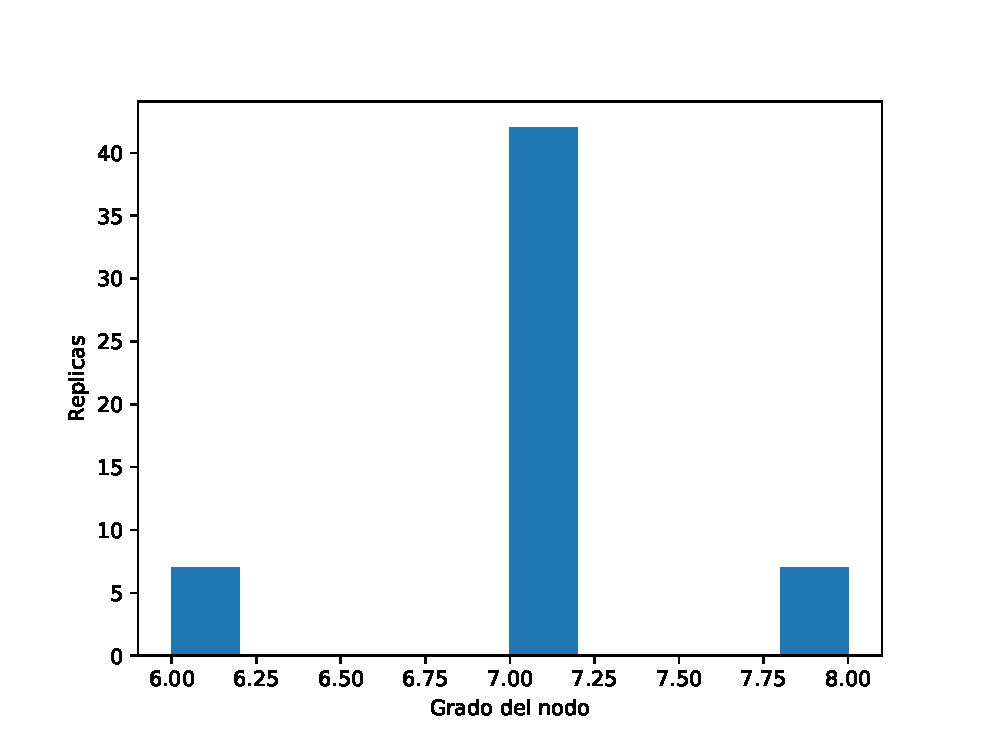
\includegraphics[scale=0.6]{hist-grados-4}
    \caption{Grafo 4}
    \label{fig:matriz}
\end{figure}
\begin{figure}[H]
    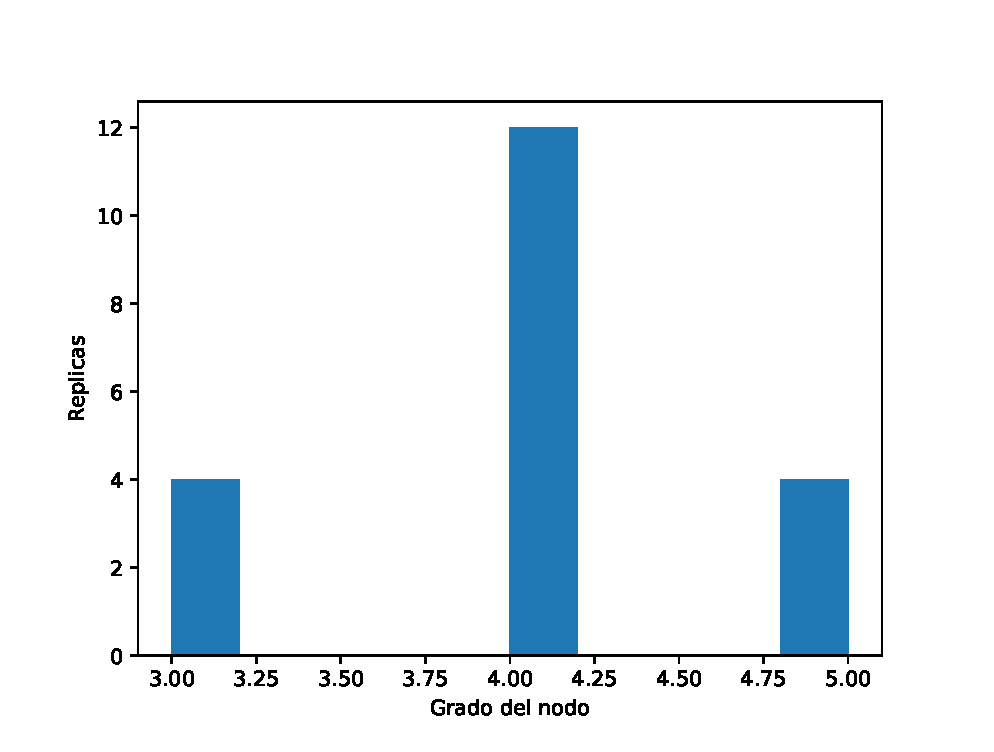
\includegraphics[scale=0.6]{hist-grados-5}
    \caption{Grafo 5}
    \label{fig:matriz}
\end{figure}

\subsection{Coeficiente de agrupamiento entre nodos}
\begin{figure}[H]
    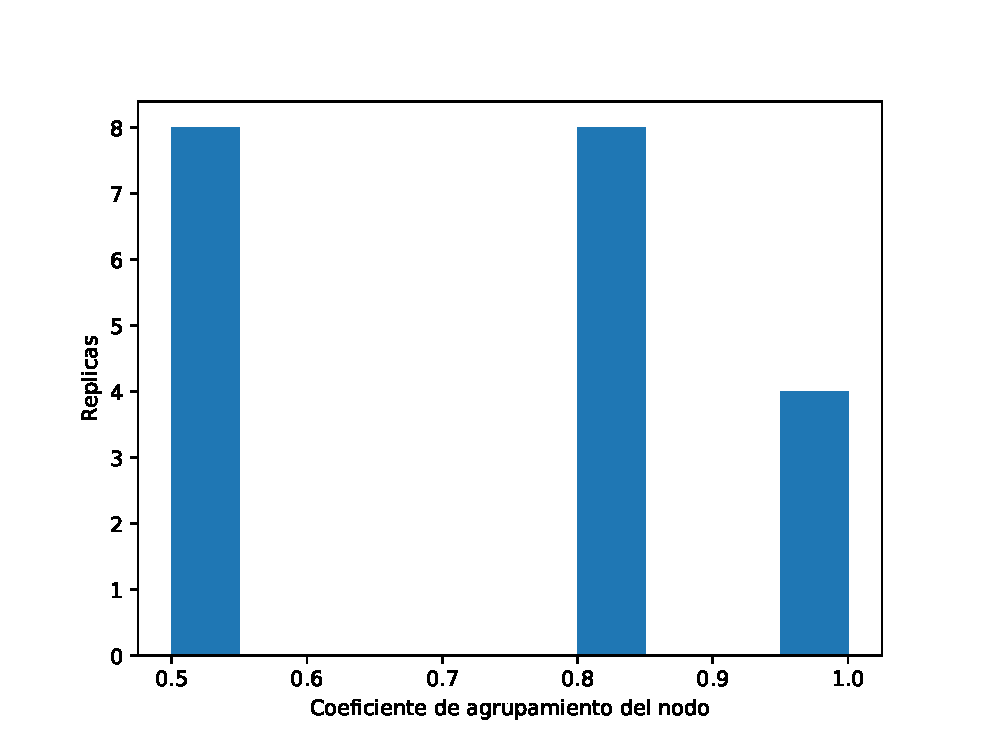
\includegraphics[scale=0.6]{hist-grado-1}
    \caption{Grafo 1}
    \label{fig:matriz}
\end{figure}
\begin{figure}[H]
    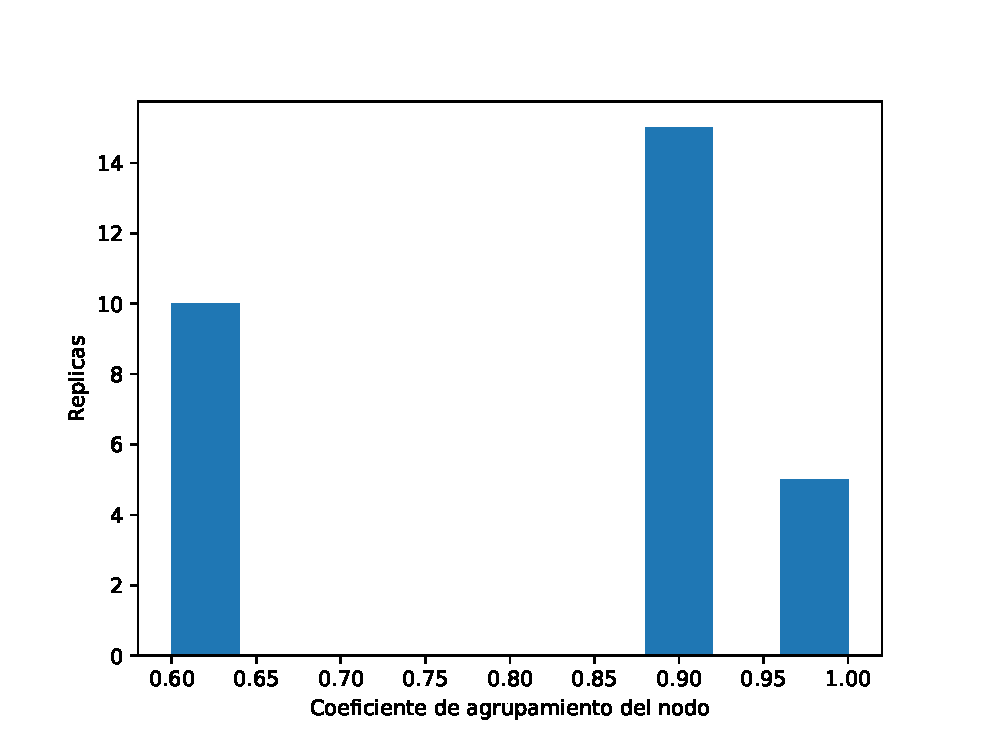
\includegraphics[scale=0.6]{hist-grado-2}
    \caption{Grafo 2}
    \label{fig:matriz}
\end{figure}
\begin{figure}[H]
    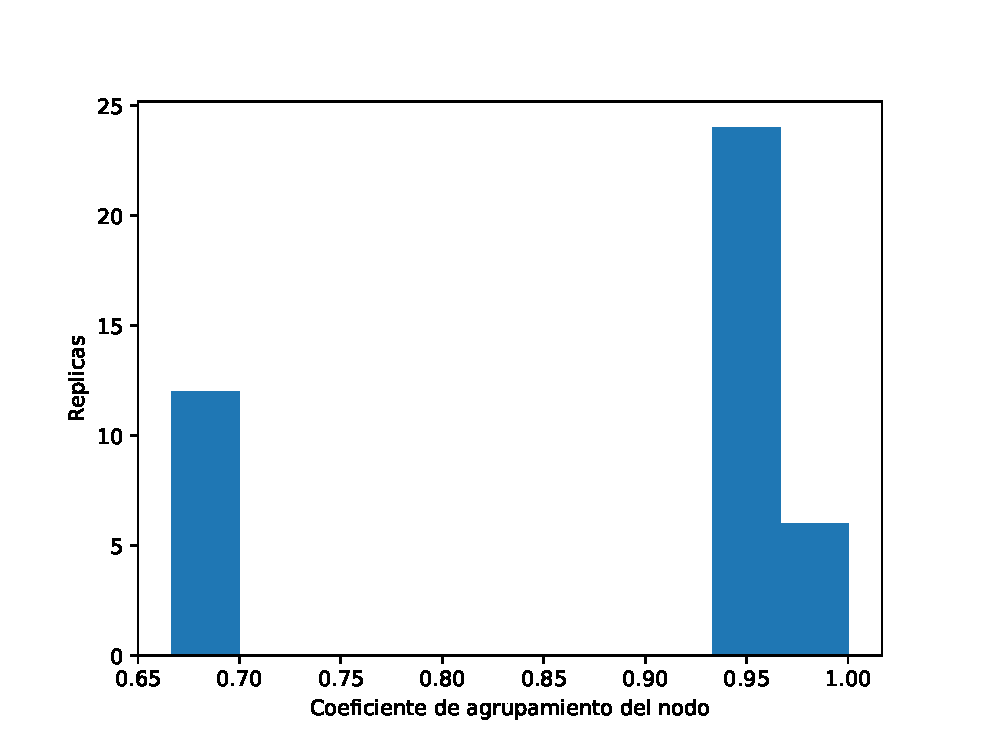
\includegraphics[scale=0.6]{hist-grado-3}
    \caption{Grafo 3}
    \label{fig:matriz}
\end{figure}
\begin{figure}[H]
    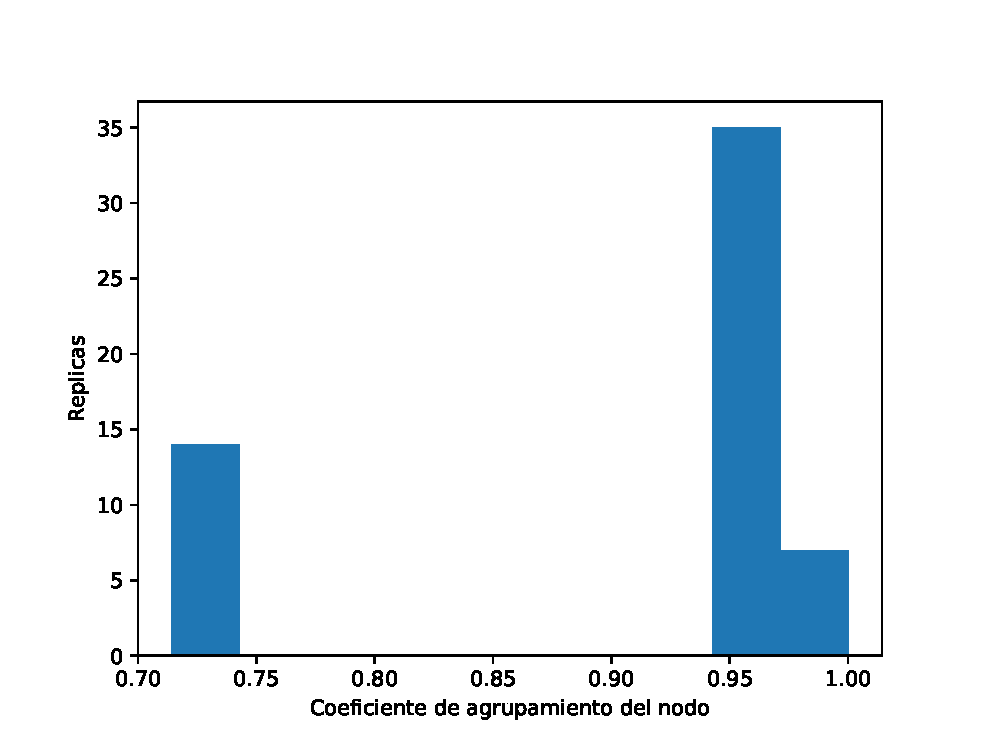
\includegraphics[scale=0.6]{hist-grado-4}
    \caption{Grafo 4}
    \label{fig:matriz}
\end{figure}
\begin{figure}[H]
    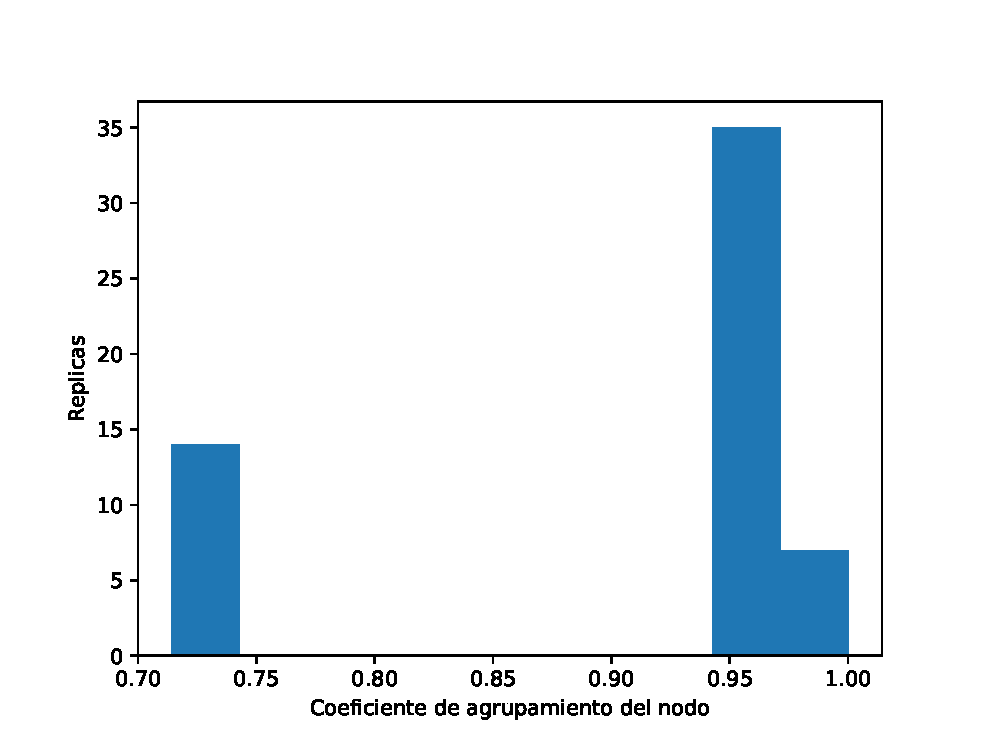
\includegraphics[scale=0.6]{hist-grado-5}
    \caption{Grafo 5}
    \label{fig:matriz}
\end{figure}

\subsection{Centralidad de cercanía entre nodos}
\begin{figure}[H]
    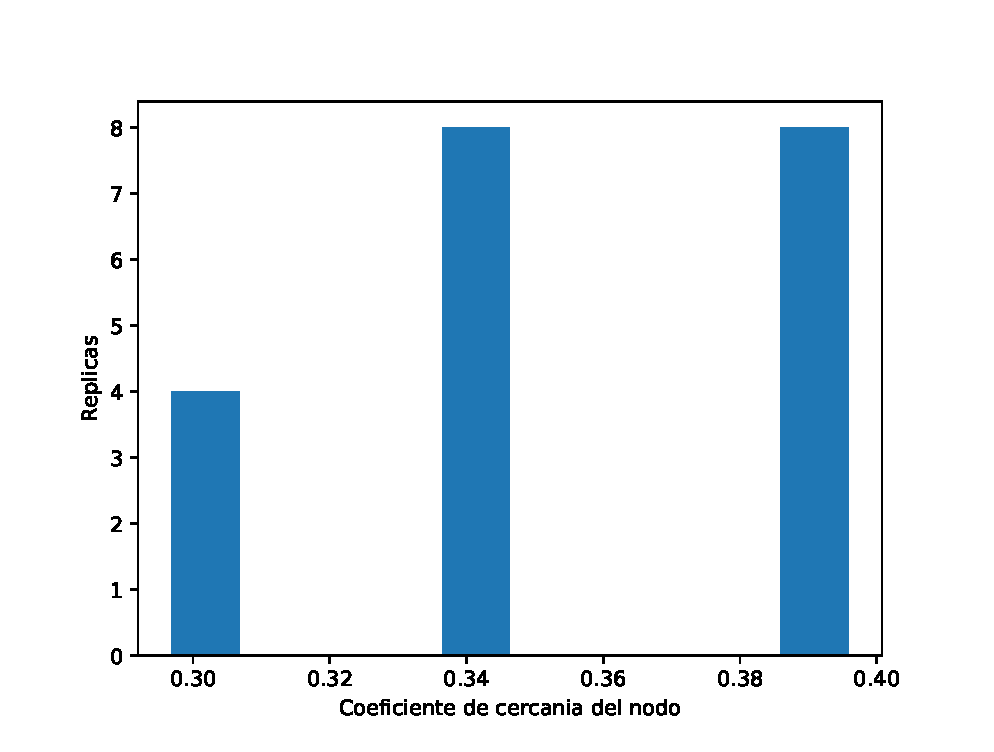
\includegraphics[scale=0.6]{hist-agrupamiento-1}
    \caption{Grafo 1}
    \label{fig:matriz}
\end{figure}
\begin{figure}[H]
    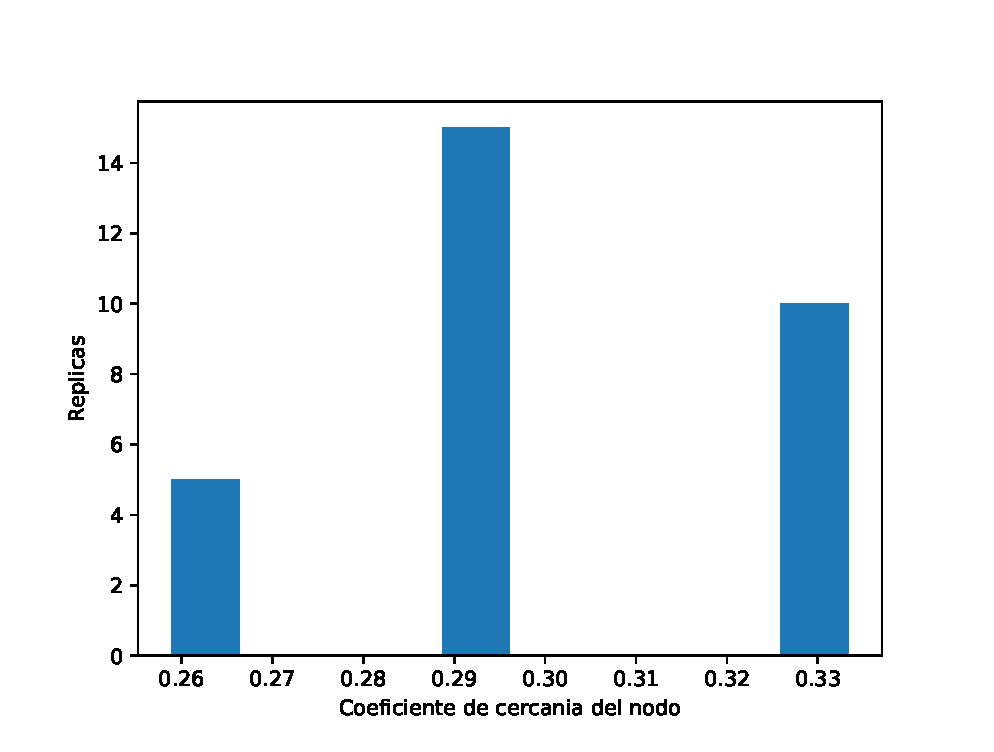
\includegraphics[scale=0.6]{hist-agrupamiento-2}
    \caption{Grafo 2}
    \label{fig:matriz}
\end{figure}
\begin{figure}[H]
    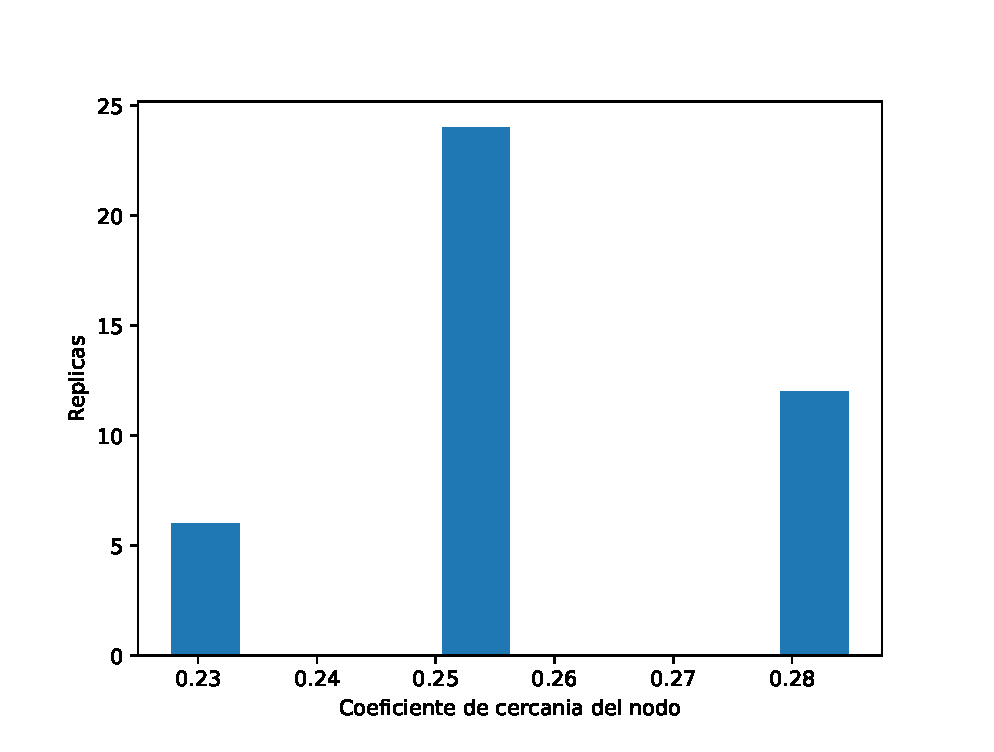
\includegraphics[scale=0.6]{hist-agrupamiento-3}
    \caption{Grafo 3}
    \label{fig:matriz}
\end{figure}
\begin{figure}[H]
    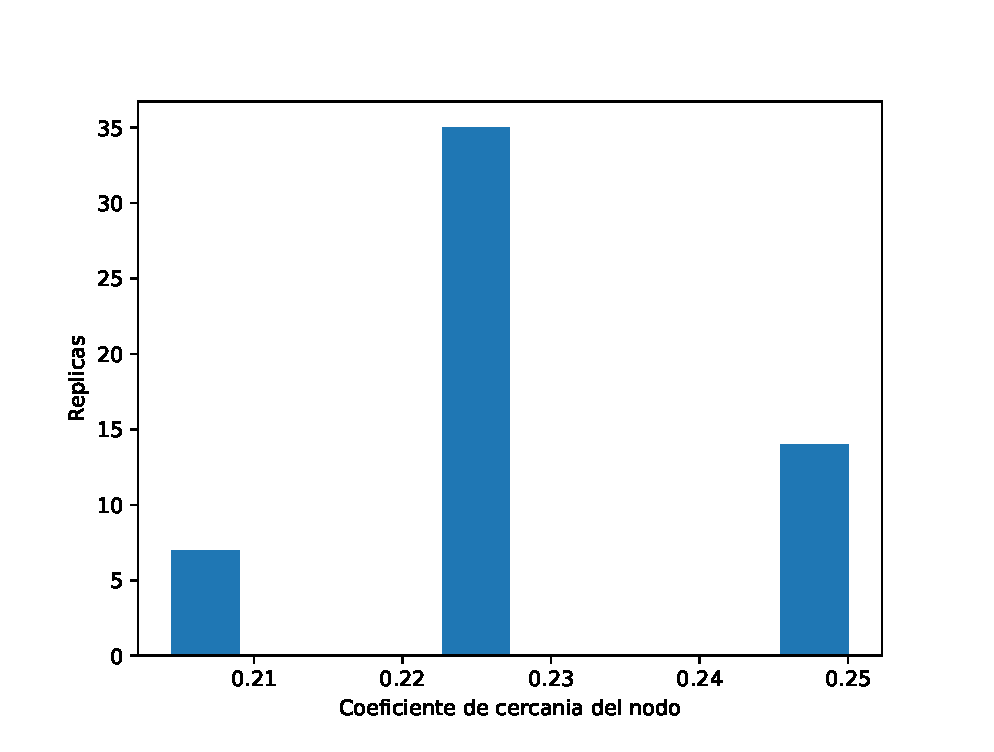
\includegraphics[scale=0.6]{hist-agrupamiento-4}
    \caption{Grafo 4}
    \label{fig:matriz}
\end{figure}
\begin{figure}[H]
    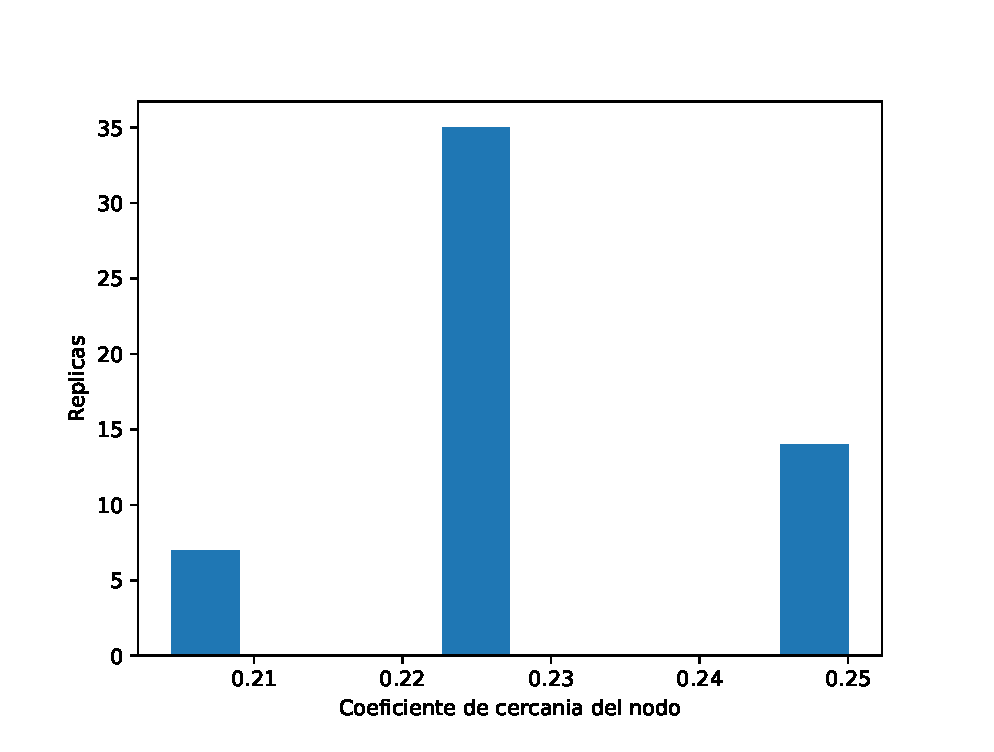
\includegraphics[scale=0.6]{hist-agrupamiento-5}
    \caption{Grafo 5}
    \label{fig:matriz}
\end{figure}

\subsection{Centralidad de carga entre nodos}
\begin{figure}[H]
    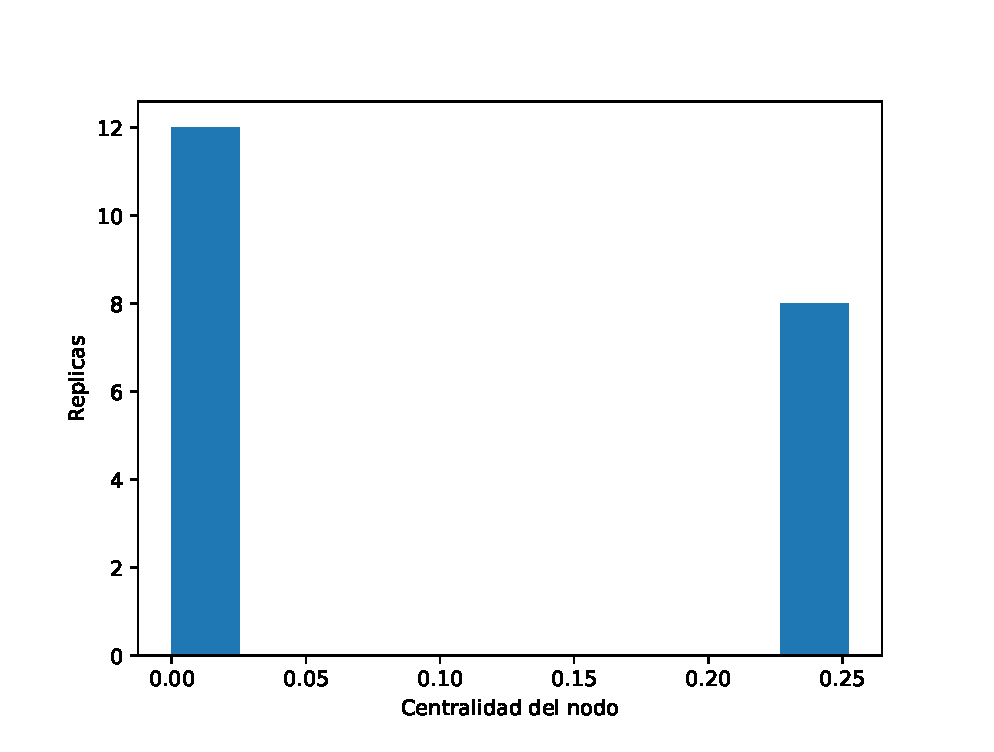
\includegraphics[scale=0.6]{hist-cercania-1}
    \caption{Grafo 1}
    \label{fig:matriz}
\end{figure}
\begin{figure}[H]
    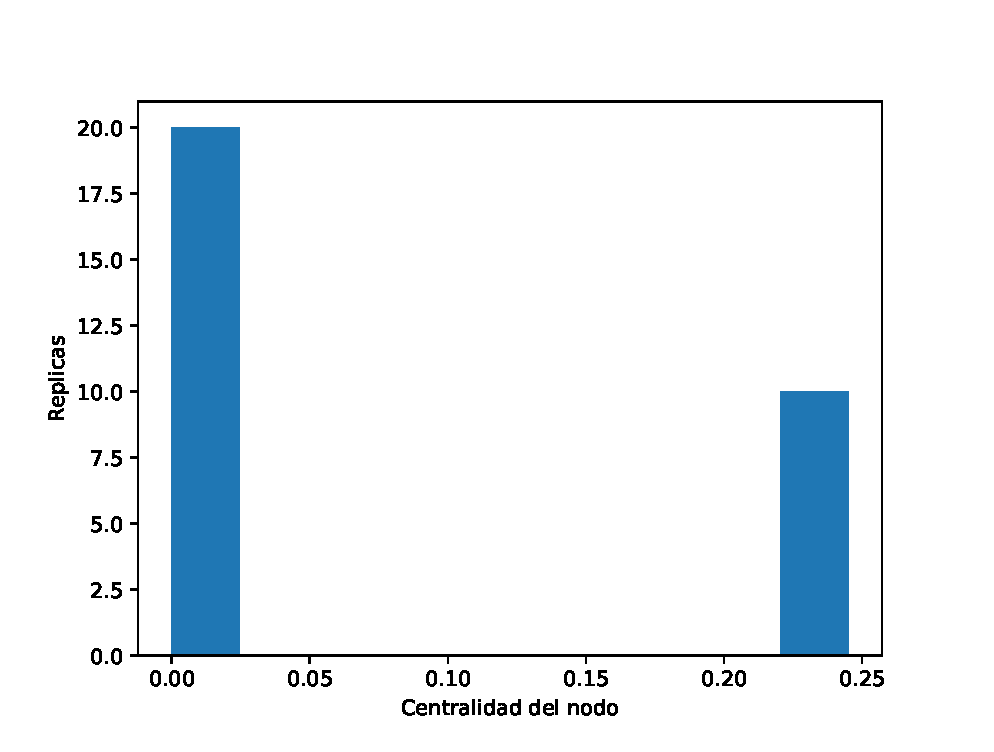
\includegraphics[scale=0.6]{hist-cercania-2}
    \caption{Grafo 2}
    \label{fig:matriz}
\end{figure}
\begin{figure}[H]
    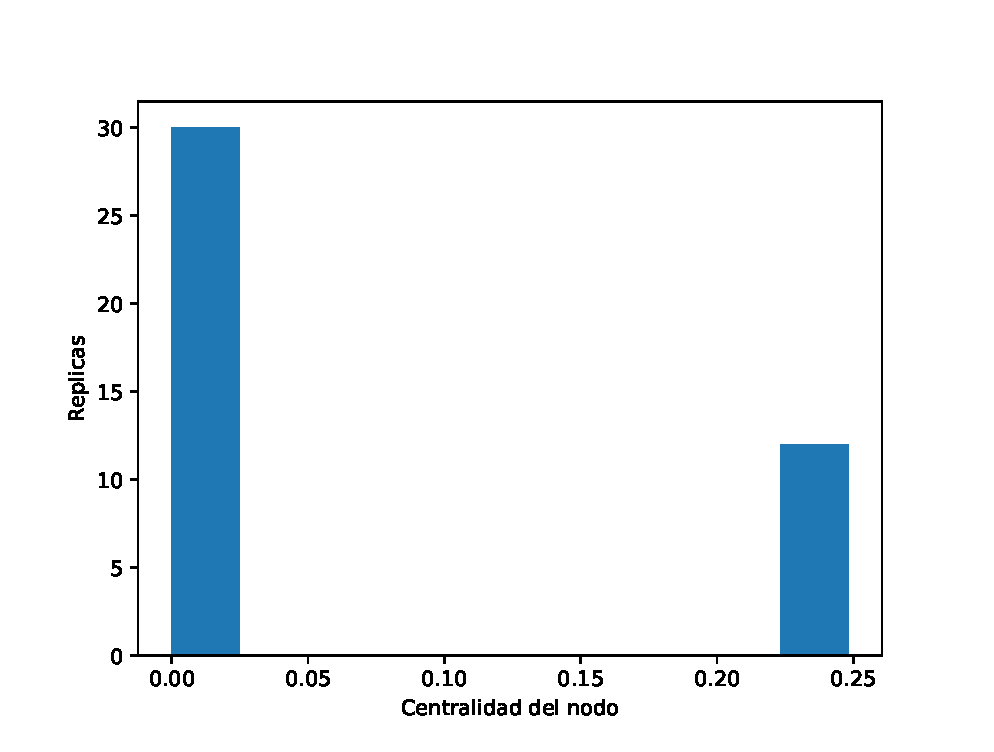
\includegraphics[scale=0.6]{hist-cercania-3}
    \caption{Grafo 3}
    \label{fig:matriz}
\end{figure}
\begin{figure}[H]
    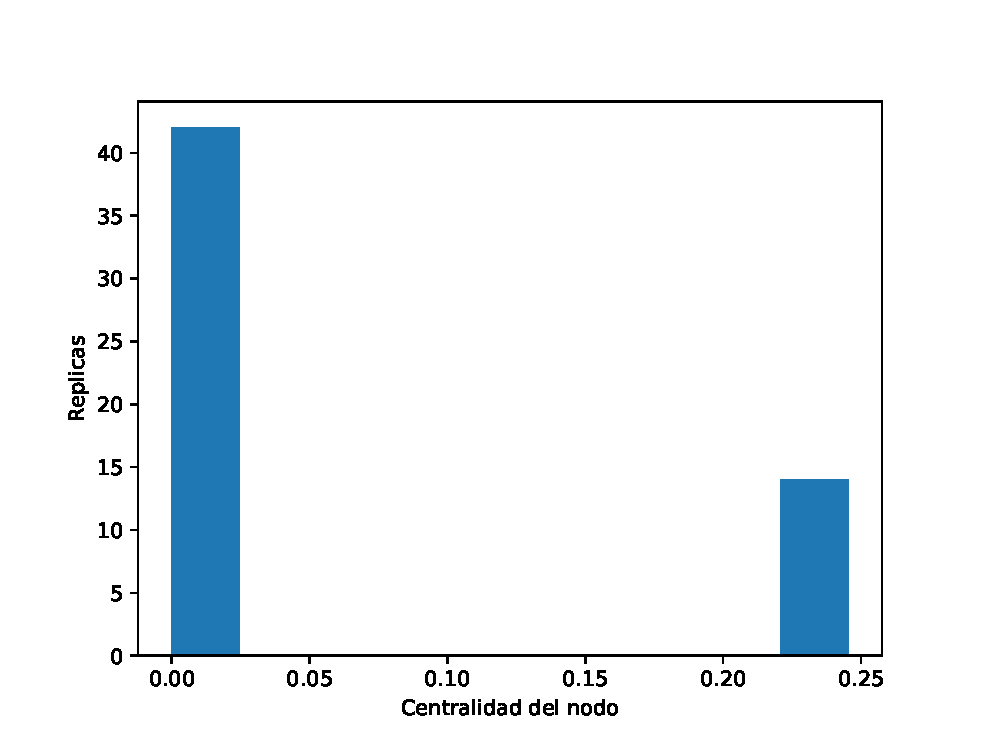
\includegraphics[scale=0.6]{hist-cercania-4}
    \caption{Grafo 4}
    \label{fig:matriz}
\end{figure}
\begin{figure}[H]
    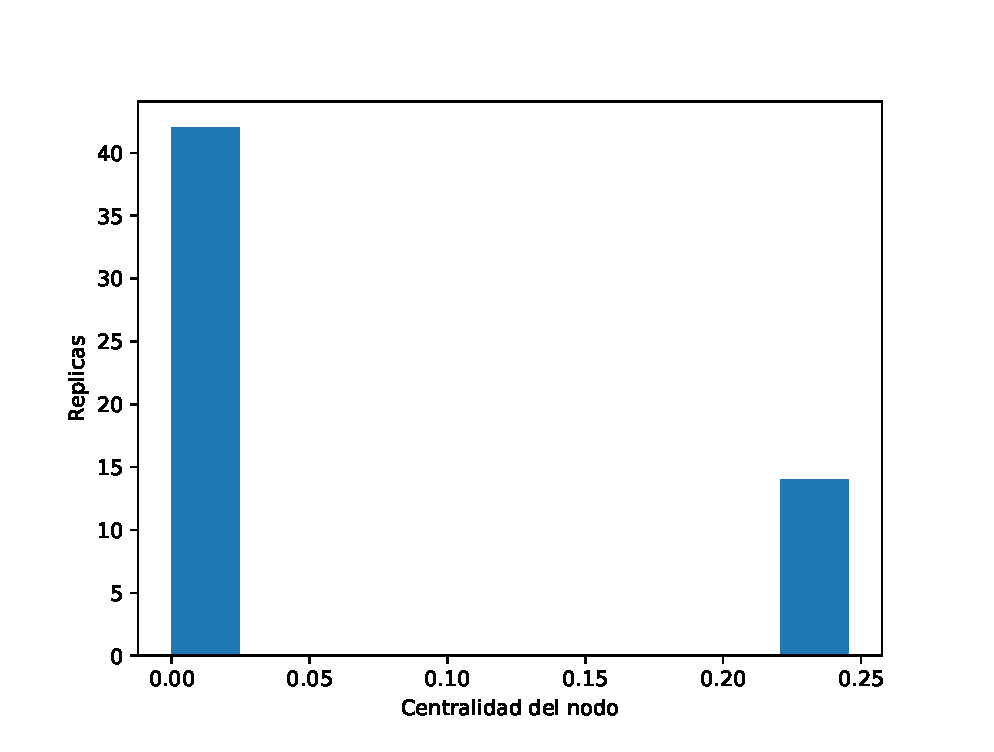
\includegraphics[scale=0.6]{hist-cercania-5}
    \caption{Grafo 5}
    \label{fig:matriz}
\end{figure}

\subsection{Excentricidad entre nodos}
\begin{figure}[H]
    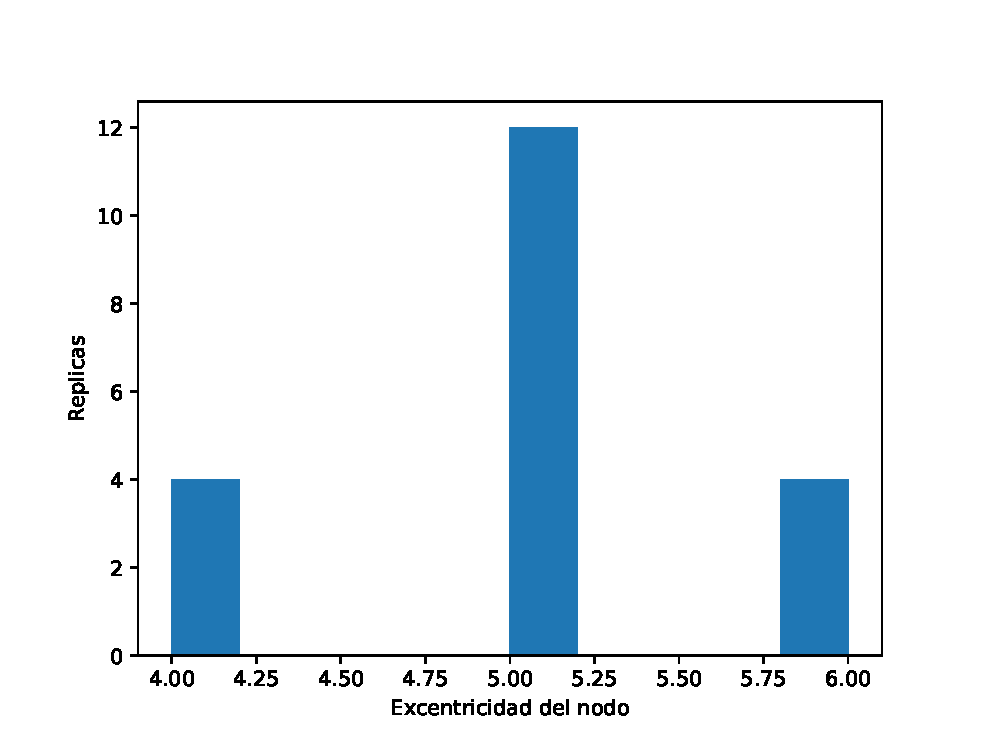
\includegraphics[scale=0.6]{hist-centralidad-1}
    \caption{Grafo 1}
    \label{fig:matriz}
\end{figure}
\begin{figure}[H]
    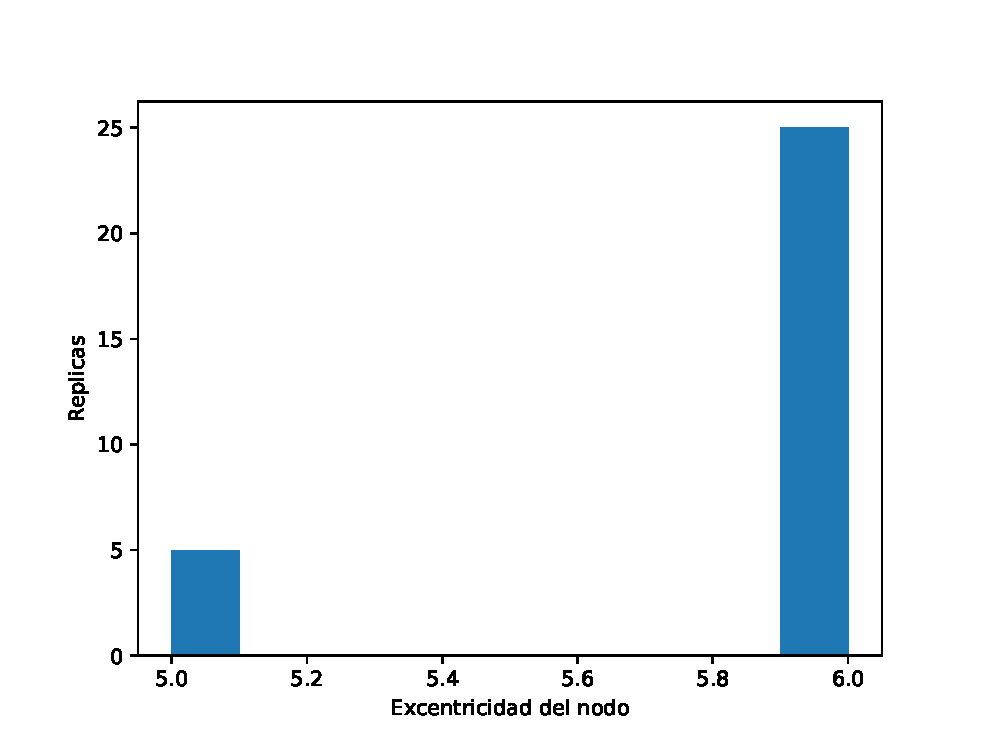
\includegraphics[scale=0.6]{hist-centralidad-2}
    \caption{Grafo 2}
    \label{fig:matriz}
\end{figure}
\begin{figure}[H]
    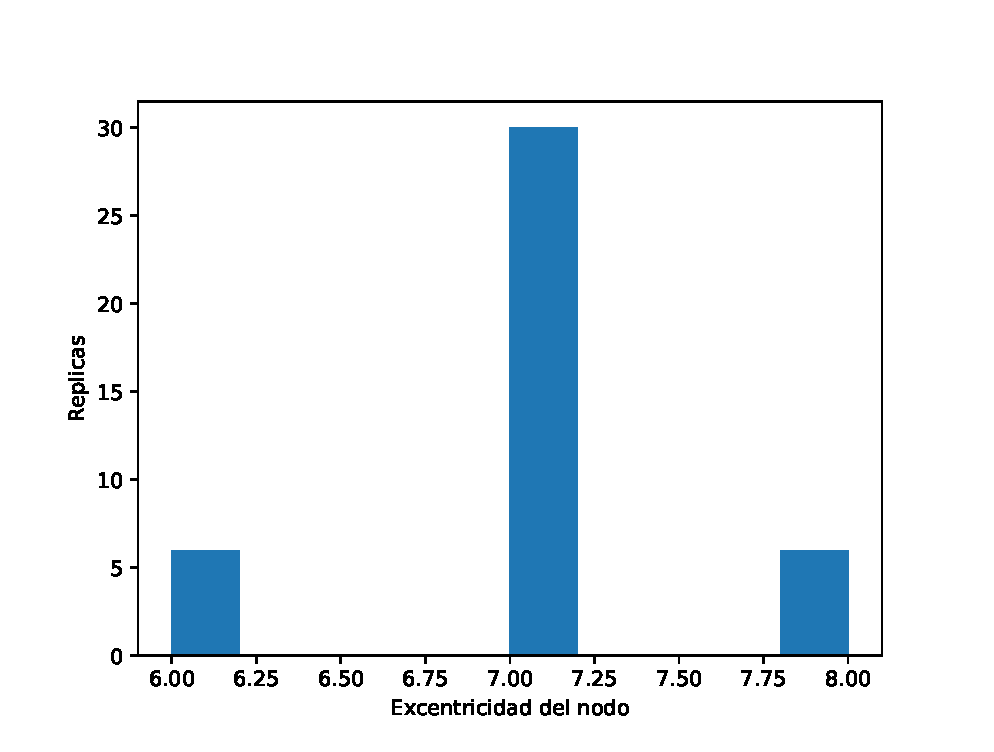
\includegraphics[scale=0.6]{hist-centralidad-3}
    \caption{Grafo 3}
    \label{fig:matriz}
\end{figure}
\begin{figure}[H]
    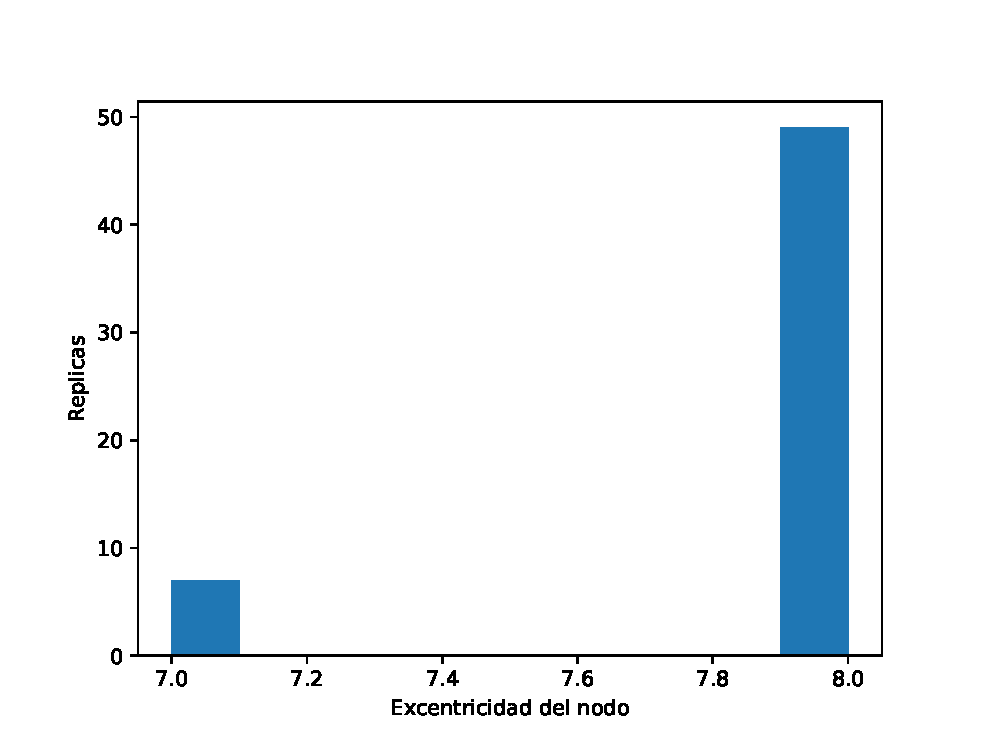
\includegraphics[scale=0.6]{hist-centralidad-4}
    \caption{Grafo 4}
    \label{fig:matriz}
\end{figure}
\begin{figure}[H]
    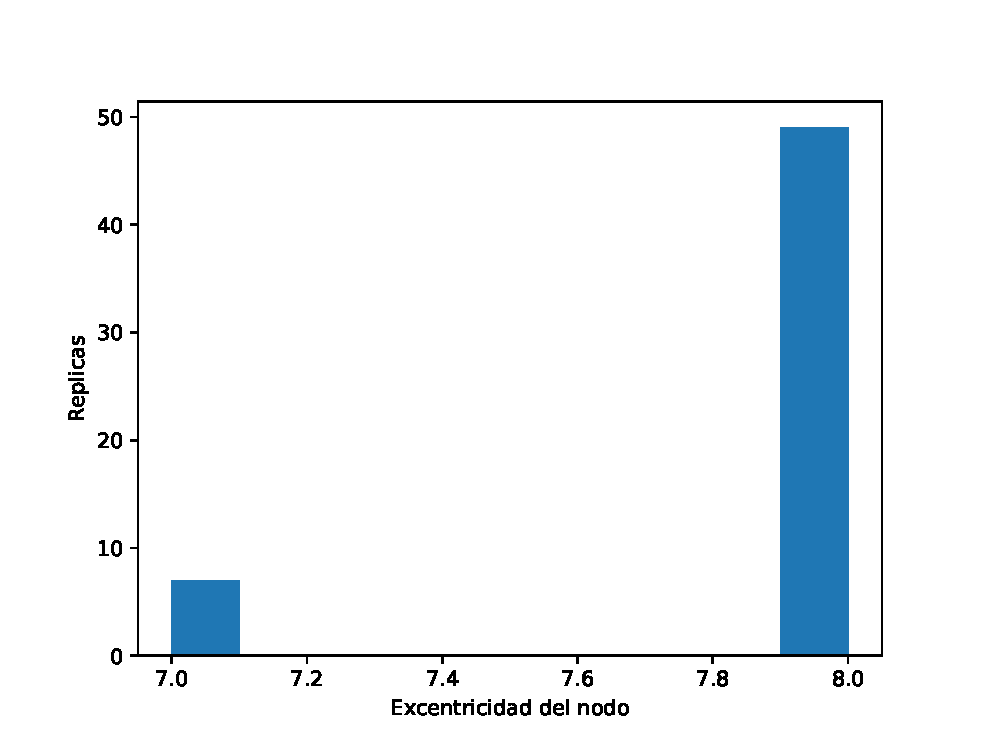
\includegraphics[scale=0.6]{hist-centralidad-5}
    \caption{Grafo 5}
    \label{fig:matriz}
\end{figure}

\subsection{PageRank entre nodos}
\begin{figure}[H]
    
\includegraphics[scale=0.6]{hist-excentricidad-1}
    \caption{Grafo 1}
    \label{fig:matriz}
\end{figure}
\begin{figure}[H]
    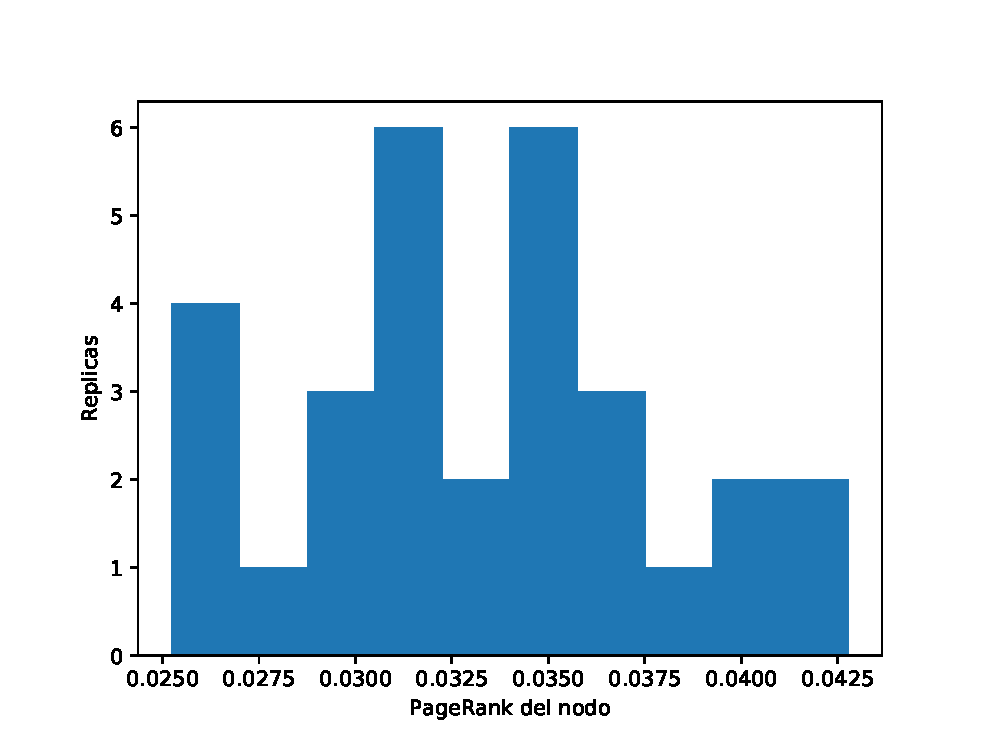
\includegraphics[scale=0.6]{hist-excentricidad-2}
    \caption{Grafo 2}
    \label{fig:matriz}
\end{figure}
\begin{figure}[H]
    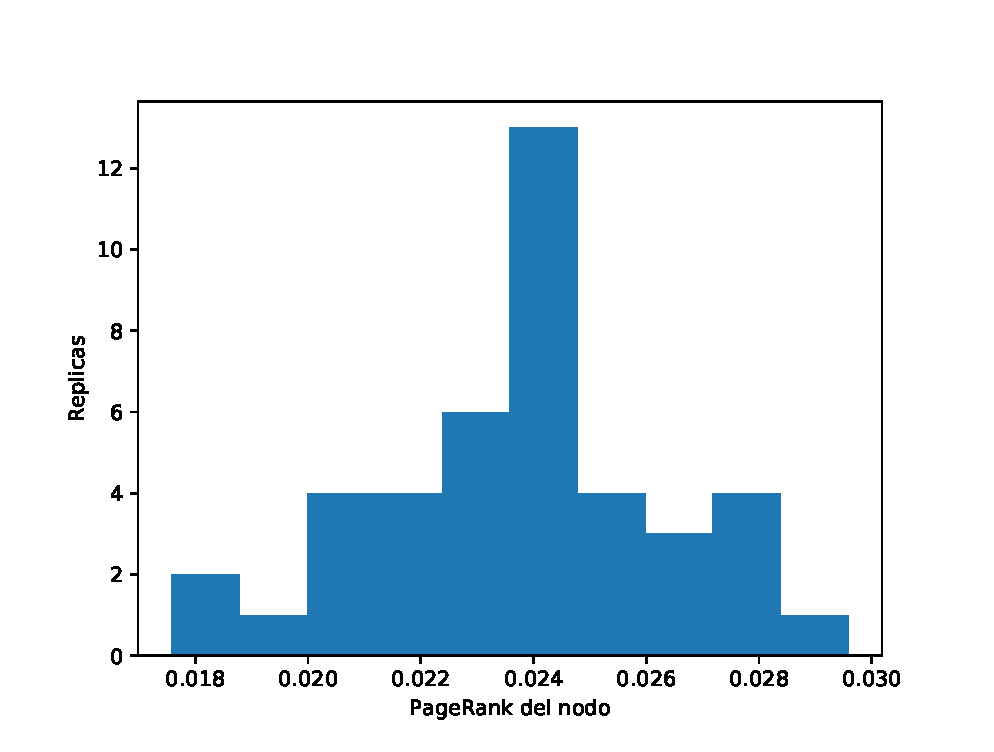
\includegraphics[scale=0.6]{hist-excentricidad-3}
    \caption{Grafo 3}
    \label{fig:matriz}
\end{figure}
\begin{figure}[H]
    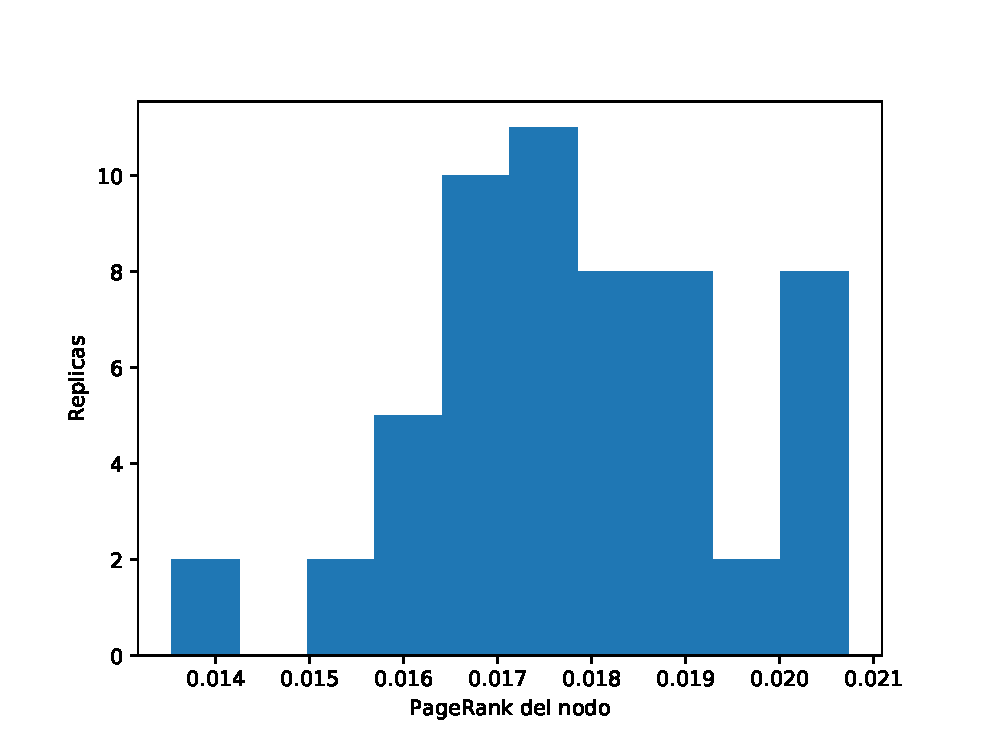
\includegraphics[scale=0.6]{hist-excentricidad-4}
    \caption{Grafo 4}
    \label{fig:matriz}
\end{figure}
\begin{figure}[H]
    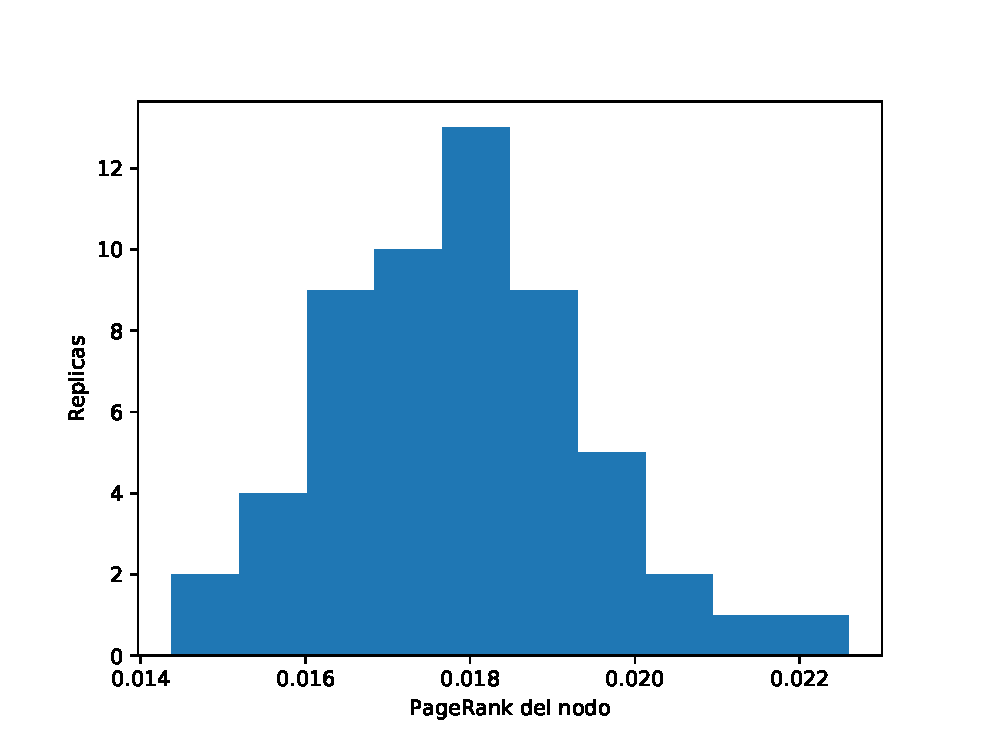
\includegraphics[scale=0.6]{hist-excentricidad-5}
    \caption{Grafo 5}
    \label{fig:matriz}
\end{figure}
Se obtuvieron los siguientes resultados de las replicas, las pruebas estadísticas de ANOVA para determinar los efectos de los factores:
\begin{figure}[H]
    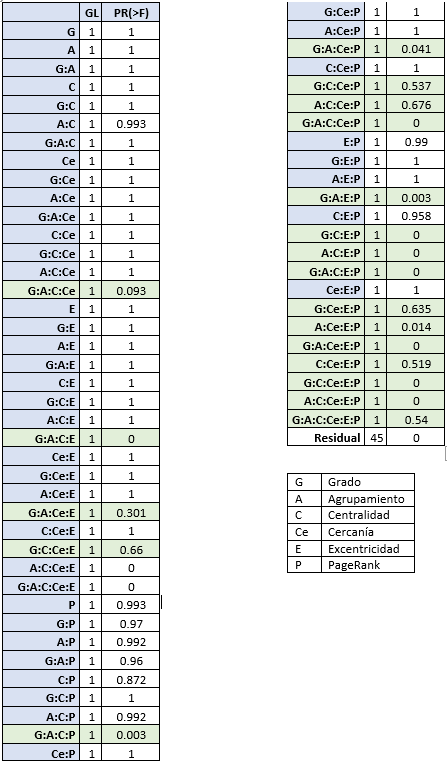
\includegraphics[width=\textwidth]{resultados}
    \label{fig:matriz}
\end{figure}

\section{Conclusiones}
Como conclusión de esta investigación, se tiene que es solamente en combinación de las características estudiadas cuando afecta el rendimiento de tiempo de ejecución del algoritmo de flujo máximo, particularmente el PageRank es la característica que más afecta en combinación con otros. La tabla ANOVA respalda los resultados con los valores de P dados.

\bibliographystyle{plain}
\bibliography{references}

\end{document}
